\documentclass[border=10pt]{standalone}
\usepackage{pgfplots}
\pgfplotsset{compat=1.18}
\begin{document}
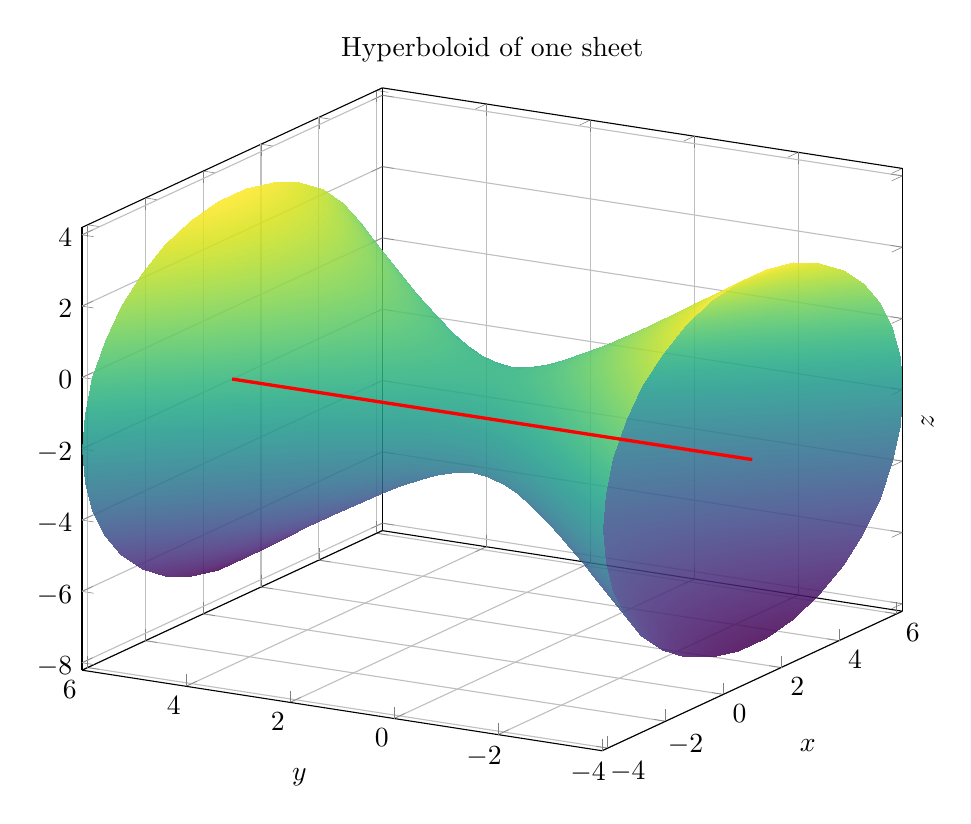
\begin{tikzpicture}
\begin{axis}[
  width=12cm, height=10cm,
  xlabel={$x$}, ylabel={$y$}, zlabel={$z$},
  title={Hyperboloid of one sheet},
  view={-60}{20},
  grid=major,
  domain=0:2*pi,
  y domain=-4:6,
  samples=35,
  samples y=25,
  colormap/viridis,
  zlabel style={at={(axis description cs:1.05,.5)}}
]
\addplot3[surf, shader=interp, opacity=0.85]
({1 + sqrt(2 + (y-1)^2)*cos(deg(x))},
 {y},
 {-2 + sqrt(2 + (y-1)^2)*sin(deg(x))});
\addplot3[red, very thick, samples y=0] coordinates {(1,-4,-2) (1,6,-2)};
\end{axis}
\end{tikzpicture}
\end{document}